% =====================================================================
%  Documento final de proyecto de grado
%  Sistema colaborativo de robots móviles para asistencia de orientación
%  en entornos interiores con múltiples pisos
%
%  Santiago Hernández Ávila · Jonny Alejandro Mejía León
%  Universidad Santo Tomás — Facultad de Ingeniería Electrónica
%
%  CÓMO SE COMPILA
%  ---------------
%  En Overleaf: subir la carpeta entera y compilar con pdfLaTeX. La bibliografía
%  usa biblatex+biber, que Overleaf ejecuta solo.
%  En local:  pdflatex main  →  biber main  →  pdflatex main  →  pdflatex main
%             (es 'biber', NO 'bibtex')
%
%  CÓMO SE TRABAJA
%  ---------------
%  Cada capítulo es un archivo aparte en capitulos/. Así dos personas pueden
%  escribir a la vez sin pisarse y cada cambio se ve en el diff de git, que es
%  justamente lo que el .docx no permitía.
%
%  El formato vive en usta-proyecto-grado.sty, con la decisión de norma
%  explicada en su cabecera. No meter ajustes de formato aquí.
% =====================================================================
\documentclass[12pt,letterpaper,oneside]{report}
\usepackage{usta-proyecto-grado}

% ---------------------------------------------------------- bibliografía ---
\addbibresource{referencias.bib}

% ------------------------------------------------------ datos del trabajo ---
\ustatitulo{Sistema colaborativo de robots móviles para asistencia de
            orientación en entornos interiores con múltiples pisos}
\ustasubtitulo{}                    % la plantilla pide aquí la relación con el objetivo general
\ustaautores{Santiago Hernández Ávila\\[0.3cm] Jonny Alejandro Mejía León}
\ustamodalidad{Proyecto de Investigación}
% Se usa el nombre que ya llevan el anteproyecto y los ocho entregables
% semanales, por coherencia con lo ya emitido y porque encaja con el acrónimo
% (GED: E = Estudio). Queda pendiente confirmarlo con el director: si el nombre
% oficial fuera «Investigación y Desarrollo», habría que corregirlo aquí Y en
% todos los documentos anteriores, no solo en este.
\ustagrupo{GED — Grupo de Estudio y Desarrollo en Robótica}
\ustalinea{Robótica y Sistemas Autónomos}   % CONFIRMAR el nombre exacto de la línea
\ustadirector{Ing. Armando Mateus Rojas, MSc.}
\ustacodirector{Ing. Néstor Iván Ospina, MSc.\\ Ing. Óscar Mauricio Gélvez Lizarazo, MSc.}
\ustaasesor{}                        % vacío = no se imprime el bloque
\ustaanio{2026}
\ustames{octubre}

\begin{document}

% =====================================================================
%  PRELIMINARES
% =====================================================================
\pagenumbering{roman}

\ustaportada
\ustacontraportada
% Autoridades académicas. Los nombres los publica la Universidad; hay que
% verificarlos en la página institucional antes de entregar, no copiarlos de
% una plantilla que puede estar desactualizada.
\ustaseccion{Autoridades académicas}

\begin{center}
P. NOMBRES COMPLETOS, O.P.\\ \textit{Rector General}\\[0.7cm]
P. NOMBRES COMPLETOS, O.P.\\ \textit{Vicerrector Administrativo y Financiero General}\\[0.7cm]
P. NOMBRES COMPLETOS, O.P.\\ \textit{Vicerrector Académico General}\\[0.7cm]
NOMBRE COMPLETO\\ \textit{Secretaria General}\\[0.7cm]
P. NOMBRES COMPLETOS, O.P.\\ \textit{Director de División de Ingenierías}\\[0.7cm]
NOMBRE COMPLETO\\ \textit{Secretaria de División de Ingenierías}\\[0.7cm]
NOMBRE COMPLETO\\ \textit{Decano Facultad de Ingeniería Electrónica}
\end{center}

\vspace{1em}
\begin{notarevisor}
Faltan por completar tres datos institucionales que no se deben transcribir de
una plantilla, porque cambian y una equivocación aquí se ve en la primera
página:

\begin{enumerate}[leftmargin=*,nosep]
  \item Los nombres de esta página, que la Universidad publica y hay que
    verificar en la fuente oficial antes de entregar.
  \item El nombre del grupo de investigación. Se usa «GED — Grupo de Estudio y
    Desarrollo en Robótica», que es el que llevan el anteproyecto y los ocho
    entregables semanales. Si el oficial fuera «Investigación y Desarrollo»,
    habría que corregirlo en todos ellos y no solo aquí.
  \item La línea de investigación. La portada dice «Robótica y Sistemas
    Autónomos» y falta confirmar la denominación exacta con el director.
\end{enumerate}
\end{notarevisor}

\ustanotaaceptacion
\ustaadvertencia
% DEDICATORIA y AGRADECIMIENTOS son OPCIONALES según la plantilla.
% Si no se usan, comentar el \input correspondiente en main.tex.
\ustaseccion{Dedicatoria}

% Homenaje a una o más personas. Una página por autor si son varios.

\ustaseccion{Agradecimientos}

% Personas e instituciones que contribuyeron: apoyo económico, toma de datos,
% préstamo de literatura y equipo, sugerencias, lectura crítica.

\vspace{1.5em}
\textbf{Conflicto de intereses}

Los autores declaran no tener ningún conflicto de intereses. Los patrocinadores
no participaron en el diseño del estudio, la recopilación, el análisis ni la
interpretación de los datos publicados, ni en la redacción del documento.

% =====================================================================
%  RESUMEN Y ABSTRACT
%  La plantilla fija 150-250 palabras y pide objetivo, método, resultados y
%  discusión. Las palabras clave son obligatorias en los dos idiomas.
% =====================================================================
\ustaseccion{Resumen}

Orientarse en un edificio de varios pisos es difícil para quien no lo conoce, y
el cambio de nivel corta la continuidad del recorrido. Las soluciones robóticas
existentes resuelven ese salto dotando al robot de mecanismos para subir
escaleras o conectándolo al ascensor, dos vías caras que obligan a intervenir la
infraestructura. Este trabajo propone y evalúa una alternativa: un sistema
colaborativo de dos robots móviles terrestres, cada uno dedicado a una planta,
que se reparten el guiado de una persona mediante un protocolo de relevo en la
zona de escaleras. Ningún vehículo cruza de nivel. La arquitectura es
centralizada: un coordinador asigna el agente según el nivel del origen y del
destino, y el usuario solicita el servicio desde una interfaz web que funciona en
cualquier teléfono sin instalación ni acceso a internet. La evaluación siguió un
protocolo escrito antes de instrumentar el sistema, con cuatro métricas de
definición operativa y treinta misiones sorteadas en simulación. La campaña
resultó válida sin descartes y permite afirmar, con 95~\% de confianza, que la
tasa de éxito supera el 70~\%. Sobre los vehículos físicos se verificó la cadena
completa de navegación y la odometría cumplió su criterio, con error entre
$-4{,}6$~\% y $+3{,}3$~\% sobre recorridos de 6,7 y 14,6~m. La precisión de
llegada quedó fuera de la tolerancia por una limitación medida de la plataforma:
el vehículo no admite velocidades por debajo de 0,40~m/s y carece de régimen de
aproximación fina.

\vspace{1em}
\textbf{Palabras clave:} robótica móvil colaborativa; sistemas multi-robot;
navegación en interiores; protocolo de relevo; interacción humano-robot; ROS~2.

\ustaseccion{Abstract}

Finding one's way inside a multi-storey building is hard for first-time
visitors, and changing floors breaks the continuity of the route. Existing
robotic solutions address that gap either by equipping the robot to climb stairs
or by interfacing it with the building lift, two expensive approaches that
require modifying the infrastructure. This work proposes and evaluates an
alternative: a collaborative system of two ground mobile robots, each assigned to
one floor, that share the task of guiding a person through a handover protocol at
the stairwell. Neither vehicle crosses between levels. The architecture is
centralised: a coordinator assigns the agent according to the floor of the origin
and the destination, and the user requests the service from a web interface that
runs on any phone with no installation and no internet access. The evaluation
followed a protocol written before instrumenting the system, with four
operationally defined metrics and thirty randomised missions in simulation. The
campaign was valid with no discards and supports, with 95~\% confidence, the
claim that the success rate exceeds 70~\%. On the physical vehicles the full
navigation chain was verified and the odometry met its criterion, with errors
between $-4{,}6$~\% and $+3{,}3$~\% over runs of 6.7 and 14.6~m. Arrival accuracy
fell outside tolerance because of a measured platform limitation: the vehicle
does not accept commanded speeds below 0.40~m/s and therefore has no fine
approach regime.

\vspace{1em}
\textbf{Keywords:} collaborative mobile robotics; multi-robot systems; indoor
navigation; handover protocol; human-robot interaction; ROS~2.

% =====================================================================
%  GLOSARIO Y ABREVIATURAS
%
%  POR QUE ESTE GLOSARIO NO REPITE EL MARCO CONCEPTUAL
%  ---------------------------------------------------
%  El §2.2 define cincuenta términos agrupados por tema, y es el lugar donde se
%  explican a fondo. Un glosario que los copiara sería redundante, y la
%  redundancia ya se había señalado como problema del documento.
%
%  Este glosario tiene otra función: permitir leer el resumen y la introducción
%  SIN haber llegado al capítulo 2. Por eso trae solo los términos que aparecen
%  antes de ese capítulo, en orden alfabético, con la definición mínima que hace
%  falta, y remite al §2.2 para el desarrollo.
%
%  La plantilla sugiere ubicarlo como anexo. Se deja en los preliminares porque
%  es donde lo pone su propia tabla de contenido, y porque un glosario que se
%  lee después del documento no cumple su función.
% =====================================================================
\ustaseccion{Glosario}

Los términos siguientes se usan desde el resumen y la introducción. El
capítulo~2 los desarrolla y añade los demás.

\begin{description}[style=nextline,leftmargin=1.5em,itemsep=0.2em]
  \item[Agente] Cada uno de los dos robots del sistema. Se usa «agente» y no
    «robot» cuando importa su papel dentro de la coordinación y no su hardware.

  \item[AMCL] Algoritmo de localización por filtro de partículas. Combina la
    odometría con las lecturas del láser para situar al robot dentro de un mapa
    que ya conoce. No construye el mapa: lo supone dado.

  \item[Banda muerta de tracción] Rango de velocidades ordenadas en el que el
    vehículo no llega a moverse, porque la señal resultante no vence el
    rozamiento estático. En la plataforma de este trabajo abarca todo lo que
    está por debajo de 0,40~m/s, y condiciona la aproximación final del vehículo
    al destino.

  \item[Cinemática tipo automóvil (dirección Ackermann)] Modelo de un vehículo
    que dirige con el eje delantero. Tiene radio de giro mínimo y no puede girar
    sobre su propio eje. Es lo contrario de la tracción diferencial, que es lo
    que la mayoría de las herramientas de navegación supone por omisión.

  \item[Continuidad del servicio] Propiedad de no interrumpir la asistencia
    mientras el usuario cambia de nivel. Es el objeto de la pregunta problema.

  \item[Localización] Estimación de la posición y la orientación del robot
    respecto a un marco de referencia fijo.

  \item[Mapa de ocupación] Cuadrícula en la que cada celda se declara libre,
    ocupada o desconocida. Es la representación del edificio con la que
    funcionan la localización y la planificación.

  \item[Mapa de costos (\textit{costmap})] Cuadrícula derivada de la anterior en
    la que cada celda lleva un costo de tránsito en lugar de una sola etiqueta.
    Permite que el planificador prefiera el centro del pasillo sin prohibir
    los bordes.

  \item[Middleware robótico] Capa de software que comunica entre sí los módulos
    del sistema. Aquí es ROS~2.

  \item[Misión] Una solicitud de guiado completa, desde que el usuario elige
    origen y destino hasta que el sistema la cierra. Es la unidad de medida de
    la campaña experimental: las métricas se reportan por misión.

  \item[Observabilidad] Propiedad de una magnitud física que permite estimarla a
    partir de las mediciones disponibles. Si en cierta combinación de entorno y
    sensor una magnitud es inobservable, ningún ajuste de parámetros la
    recupera, porque la información no está en la señal. El §2.3.4 muestra un
    caso concreto en un pasillo recto.

  \item[Odometría] Estimación del desplazamiento propio del robot a partir de
    sus propias mediciones. La plataforma de este trabajo no tiene encoders, así
    que la obtiene comparando barridos sucesivos del láser.

  \item[Punto de transferencia] Lugar físico, en este trabajo la escalera, donde
    un agente entrega el guiado y el otro lo recibe.

  \item[Relevo] Traspaso de la responsabilidad de guiar a una persona, de un
    agente al otro, en un punto acordado de antemano. Es el aporte que el
    proyecto declara, y lo que sustituye al hardware de transición vertical.

  \item[Tasa de éxito] Proporción de misiones que terminan como el protocolo
    experimental declara que deben terminar. Su definición operativa está en el
    §3.4.

  \item[Tiempo de respuesta] Intervalo entre la solicitud del usuario y el
    instante en que el robot asignado arranca la tarea.

  \item[Zona de transición] Punto del edificio donde se cambia de nivel:
    escalera o ascensor. En este sistema ningún robot la atraviesa.
\end{description}

\ustaseccion{Abreviaturas}

\begin{description}[style=nextline,leftmargin=1.5em,itemsep=0.2em]
  \item[AMCL] \textit{Adaptive Monte Carlo Localization} — localización adaptativa
    por método de Monte Carlo.
  \item[AWS] \textit{Amazon Web Services}, fabricante de la plataforma DeepRacer
    empleada como vehículo.
  \item[CONPES] Consejo Nacional de Política Económica y Social (Colombia).
  \item[DDS] \textit{Data Distribution Service} — protocolo de transporte sobre
    el que ROS~2 implementa sus comunicaciones.
  \item[GED] Grupo de Estudio y Desarrollo en Robótica, grupo de investigación en
    el que se inscribe el proyecto.
  \item[GUI] \textit{Graphical User Interface} — interfaz gráfica de usuario.
  \item[HRI] \textit{Human-Robot Interaction} — interacción humano-robot.
  \item[ICONTEC] Instituto Colombiano de Normas Técnicas y Certificación.
  \item[IMU] \textit{Inertial Measurement Unit} — unidad de medición inercial.
  \item[JSON] \textit{JavaScript Object Notation}, formato de intercambio de
    datos en texto.
  \item[MRS] \textit{Multi-Robot System} — sistema multi-robot.
  \item[Nav2] \textit{Navigation2}, marco de navegación autónoma de ROS~2.
  \item[NTC] Norma Técnica Colombiana.
  \item[OE] Objetivo específico. Los cuatro del proyecto están en el §1.3.2 y
    organizan los capítulos~3 y~4.
  \item[PID] Control proporcional-integral-derivativo.
  \item[PWM] \textit{Pulse Width Modulation} — modulación por ancho de pulso.
  \item[QoS] \textit{Quality of Service} — políticas de entrega de un canal de
    comunicación.
  \item[RF] Requisito funcional. La numeración RF-\textit{nn} remite a la
    especificación de requisitos del sistema.
  \item[ROS] \textit{Robot Operating System}. La versión empleada es ROS~2, que
    no es una actualización de ROS~1 sino un rediseño sobre DDS.
  \item[SLAM] \textit{Simultaneous Localization and Mapping} — localización y
    mapeo simultáneos.
\end{description}


% ------------------------------------------------------------- índices ---
\ustaseccion{Contenido}
\tableofcontents

\ustaseccion{Lista de figuras}
\listoffigures

% Gráficas: tipo flotante propio, definido en el .sty. La plantilla las
% distingue de las figuras («una gráfica contiene ejes coordenados»).
\ustaseccion{Lista de gráficas}
\listofgraficas

\ustaseccion{Lista de tablas}
\listoftables

\ustaseccion{Lista de códigos}
\lstlistoflistings

% =====================================================================
%  CUERPO
% =====================================================================
\clearpage
\pagenumbering{arabic}
\setcounter{page}{1}

% =====================================================================
%  INTRODUCCIÓN
%  La plantilla la quiere como párrafos continuos (sin subsecciones) que
%  cubran: planteamiento, antecedentes, propósito, fundamentación, pregunta
%  de investigación, justificación (impacto y beneficiarios) y el enfoque
%  empleado para resolver el problema.
%
%  DE DÓNDE SALE LO QUE YA ESTÁ ESCRITO
%    Anteproyecto cap. 1 (Introducción) y cap. 3 (Justificación)
%    → Documentos/Anteproyecto_Jonny_Santi.pdf
% =====================================================================
\chapter*{Introducción}
\addcontentsline{toc}{chapter}{INTRODUCCIÓN}

% PENDIENTE

% =====================================================================
%  CONTEXTUALIZACIÓN
%  Los objetivos se transcriben LITERAL del anteproyecto §4.1 y §4.2: son los
%  aprobados y no se reescriben.
% =====================================================================
\chapter{Contextualización}

\section{Planteamiento del problema}

Orientarse en un edificio desconocido exige construir y actualizar una
representación mental del espacio. El proceso se complica cuando el entorno tiene
visibilidad limitada, estructuras repetidas y varios puntos de decisión.
\textcite{omer2025multilayer} describen esos espacios compartidos con personas
como el escenario que más exige a un robot. Vale también para quien camina sin
conocerlos.

Las edificaciones de varios pisos añaden una dificultad propia. El cambio de
nivel rompe la continuidad espacial y obliga a integrar información vertical en
el recorrido. Es el mismo problema que \textcite{kim2024indoor} resuelven para un
robot, con un grafo topológico entre plantas.

La robótica móvil colaborativa ha avanzado en exploración, logística y cobertura
distribuida. La asignación de tareas entre agentes tiene una formalización
aceptada desde el trabajo de \textcite{gerkey2004taxonomy}. Pero la mayoría de
esos desarrollos se evaluó en entornos de una sola planta, donde la segmentación
vertical no es el problema central. Los casos de limpieza doméstica y de almacén
que documenta \textcite{nair2024collaborative} son representativos de ese
escenario plano.

Resolver el cambio de piso con un solo robot resulta caro. Exige mecanismos de
locomoción capaces de subir escaleras, o intervenir el sistema de control del
ascensor. \textcite{song2024elevator} lo hacen instalando dispositivos conectados
en la propia cabina. Las dos opciones elevan el costo del hardware y
obligan a modificar el edificio.

De ahí el planteamiento de este trabajo. El problema no es cómo hacer que un
robot suba, sino \textbf{cómo lograr que dos robots sencillos se repartan el
recorrido y se pasen al usuario sin que la asistencia se interrumpa}. La
comunicación entre agentes sustituye al hardware de transición vertical.

\section{Pregunta problema}

\begin{quote}
¿Es viable mantener la continuidad de la asistencia de orientación a una persona
que cambia de nivel en un edificio, mediante un esquema de relevo entre dos
robots móviles dedicados cada uno a una planta, sin que ninguno de ellos
atraviese la zona de transición vertical?
\end{quote}

La pregunta tiene dos mitades y las dos se responden en el capítulo~4. La primera
es de funcionamiento: si el relevo ocurre. La segunda es de medida: con qué
incertidumbre se puede afirmar.

\section{Objetivos}

\subsection{Objetivo general}

Implementar un sistema colaborativo de dos robots móviles terrestres para la guía
coordinada y eficiente de asistencia a visitantes en entornos interiores con
múltiples pisos, mediante comunicación inter-robot, asignación dinámica de tareas
y una interfaz móvil de interacción usuario-robot.

\subsection{Objetivos específicos}

\begin{enumerate}[leftmargin=*,label=\textbf{OE\arabic*.}]
  \item Modelar la arquitectura funcional del sistema colaborativo de dos robots
    móviles, definiendo requerimientos, escenarios de operación con múltiples
    pisos, estrategia de asignación de tareas y esquema de comunicación
    inter-robot.
  \item Desarrollar una plataforma robótica móvil basada en dos vehículos tipo
    DonkeyCar, integrando los módulos de locomoción, sensado, procesamiento y
    comunicación necesarios para la operación colaborativa en entornos
    interiores.
  \item Programar una interfaz móvil para interacción humano-robot (HRI) basada
    en la selección de localizaciones de interés de origen y destino.
  \item Evaluar el desempeño del sistema mediante pruebas experimentales en un
    entorno interior controlado, utilizando métricas como tiempo de respuesta,
    tiempo de asignación de robot, tasa de éxito en la entrega de asistencia y
    continuidad del servicio entre niveles.
\end{enumerate}

Estos cuatro objetivos organizan el resto del documento. El capítulo~3 dedica una
sección a cada uno, y el~4 reporta lo que se midió para cada uno.

% =====================================================================
%  MARCO REFERENCIAL
%
%  Los §2.1 y §2.2 se trasvasan del informe de avance del marco teórico
%  (Documentos/Entregables/Actualizacion_Marco_Teorico_Conceptual.tex),
%  adaptados a la jerarquía de capítulo/sección/subsección del documento final.
%
%  Los §2.3 y §2.4 son contenido nuevo: no existían en ningún documento del
%  proyecto. Llevan marcados en comentarios los puntos que hay que VERIFICAR
%  antes de entregar; no se afirma nada normativo que no esté comprobado.
% =====================================================================
\chapter{Marco referencial}

Este capítulo reúne el vocabulario técnico, los fundamentos teóricos y el
encuadre normativo y ambiental con que opera el proyecto. Se organiza en cuatro
marcos. El conceptual fija el significado de los términos que el resto del
documento usa sin volver a definirlos. El teórico expone las decisiones de
arquitectura y sus fundamentos, incluidas aquellas que la implementación obligó
a revisar. El legal sitúa el trabajo frente a la normativa aplicable, y el
ambiental frente a las consideraciones de consumo y ciclo de vida del hardware
empleado.

% =====================================================================
\section{Marco conceptual}
% =====================================================================

Se definen a continuación los términos técnicos necesarios para la lectura del
documento, considerando un público con formación en ingeniería electrónica.
La organización en seis categorías se conserva del anteproyecto; dentro de cada
una, los términos que la implementación introdujo se añaden a los ya definidos.

\subsection{Navegación y percepción}

\begin{description}[style=nextline,leftmargin=1.5em]
  \item[Navegación autónoma] Desplazamiento sin intervención humana que integra
    percepción, localización y control.
  \item[Odometría] Estimación de posición por integración de mediciones de
    actuadores o de sensores exteroceptivos.
  \item[Zona de transición] Punto crítico para el cambio de nivel en
    edificaciones con múltiples pisos.
  \item[Mapa de costos (\textit{costmap})] Representación del entorno usada para
    la planificación, que asigna a cada celda un costo de tránsito en lugar de un
    simple estado libre u ocupado. Existe una capa global, que cubre el mapa
    completo, y una local, limitada al entorno inmediato del robot.
  \item[AMCL (\textit{Adaptive Monte Carlo Localization})] Algoritmo de
    localización basado en un filtro de partículas que estima la posición y
    orientación del robot combinando la odometría con las lecturas del sensor
    láser contra un mapa conocido.
  \item[Verificador de meta (\textit{goal checker})] Componente que decide si el
    robot alcanzó su objetivo, comparando posición y, opcionalmente, orientación
    contra una tolerancia.
  \item[Observabilidad de un estado] Propiedad de una variable física de poder
    estimarse a partir de las mediciones disponibles. Una variable puede ser
    matemáticamente inobservable en una configuración concreta de entorno y
    sensor, sin que exista error de calibración que lo corrija.
  \item[Modelo de movimiento Reeds-Shepp] Conjunto de trayectorias óptimas para
    un vehículo con curvatura acotada que puede moverse hacia adelante y hacia
    atrás, usado por el planificador híbrido para generar maniobras de inversión
    de marcha.
  \item[Cúspide] Punto de una trayectoria planificada en el que el vehículo
    invierte el sentido de marcha.
\end{description}

\subsection{Control y locomoción}

\begin{description}[style=nextline,leftmargin=1.5em]
  \item[Cinemática de robots móviles] Modelo matemático del movimiento en
    función de las velocidades de los actuadores.
  \item[Modelo cinemático tipo automóvil (dirección Ackermann)] Representación
    geométrica y matemática de un vehículo de cuatro ruedas con dirección en el
    eje delantero, como la plataforma empleada. Relaciona el ángulo de giro del
    servomotor con el radio de giro del vehículo, asegurando que las ruedas
    interior y exterior giren en torno a un mismo centro instantáneo de rotación.
  \item[PWM (\textit{Pulse Width Modulation})] Técnica para controlar motores o
    servomotores mediante el ciclo de trabajo de una señal.
  \item[Control PID] Algoritmo de control por retroalimentación
    proporcional-integral-derivativo.
  \item[Planificador híbrido A* (\textit{Smac Hybrid-A*})] Algoritmo de búsqueda
    de rutas que opera sobre el espacio continuo de posición y orientación,
    respetando las restricciones cinemáticas del vehículo, a diferencia de un
    planificador de cuadrícula que ignora la orientación.
  \item[Controlador de seguimiento regulado (\textit{Regulated Pure Pursuit})]
    Algoritmo de control que persigue un punto móvil sobre la trayectoria
    planificada, regulando su velocidad según la curvatura y la proximidad a
    obstáculos.
  \item[Banda muerta de tracción] Intervalo de velocidades comandadas por debajo
    del cual el vehículo no llega a moverse, porque la señal resultante no vence
    el rozamiento estático.
\end{description}

\subsection{Comunicación y sistemas distribuidos}

\begin{description}[style=nextline,leftmargin=1.5em]
  \item[Middleware robótico] Capa de software para la comunicación entre módulos
    del sistema.
  \item[ROS (\textit{Robot Operating System})] Middleware con nodos, tópicos de
    publicación y suscripción, servicios de petición y respuesta, y acciones
    \cite{macenski2022ros2}.
  \item[DDS (\textit{Data Distribution Service})] Protocolo de transporte de
    publicación y suscripción sobre el que ROS 2 implementa sus tópicos,
    servicios y acciones, con descubrimiento automático de participantes.
  \item[Dominio ROS] Identificador numérico que segmenta el descubrimiento DDS.
    Dos procesos con distinto dominio no se ven entre sí salvo configuración
    explícita.
  \item[Espacio de nombres (\textit{namespace})] Prefijo aplicado a los tópicos,
    servicios y acciones de un nodo, usado en este trabajo para aislar a cada
    agente dentro de un mismo dominio DDS.
  \item[Acción ROS] Patrón de comunicación asíncrona para tareas de larga
    duración, compuesto por un objetivo, retroalimentación periódica y un
    resultado final, con posibilidad explícita de cancelación.
  \item[Servidor y cliente de acción] Nodo que ofrece una acción y nodo que la
    invoca. En este sistema el coordinador es cliente de la acción de navegación
    ante cada agente y servidor de la acción de guiado ante la interfaz.
  \item[Callback de cancelación] Función que un servidor de acción debe registrar
    explícitamente para poder aceptar solicitudes de cancelación; sin ella, el
    comportamiento por omisión es rechazarlas.
  \item[Calidad de servicio (QoS)] Conjunto de políticas de entrega de un tópico
    o servicio, configurable de forma independiente para cada canal.
  \item[Puente \textit{rosbridge}] Servidor que traduce entre el protocolo nativo
    de ROS 2 y un protocolo JSON sobre WebSocket, permitiendo que un cliente web
    sin dependencias de ROS publique, se suscriba y opere acciones.
\end{description}

\subsection{Arquitectura del sistema}

\begin{description}[style=nextline,leftmargin=1.5em]
  \item[Asignación de tareas] Distribución de actividades entre robots según su
    disponibilidad y ubicación \cite{gerkey2004taxonomy}.
  \item[Protocolo de relevo] Transferencia secuencial de responsabilidad entre
    agentes en puntos definidos.
  \item[Máquina de estados de misión] Conjunto de valores discretos y ordenados
    que describen el progreso de una misión, publicados para que tanto la
    interfaz como el registro de evaluación conozcan el punto de ejecución.
  \item[Planificador puro] Componente que calcula la secuencia de tramos de una
    misión a partir del catálogo de puntos y del par origen-destino, sin depender
    del middleware ni de ningún estado externo, lo que permite verificarlo con
    cientos de casos en milisegundos y sin simulador.
  \item[Punto de transferencia] Punto de interés marcado en el catálogo como el
    lugar físico, típicamente una escalera, en el que un agente entrega y otro
    recibe la continuidad del guiado al cambiar de nivel.
  \item[Registro de misión] Documento estructurado, compuesto a partir de la
    grabación de la misión y validado contra un esquema formal, que constituye la
    evidencia primaria de una ejecución para efectos de la evaluación
    experimental.
\end{description}

\subsection{Interacción humano-robot}

\begin{description}[style=nextline,leftmargin=1.5em]
  \item[Interfaz gráfica de usuario (GUI)] Entorno visual para la interacción
    humano-máquina.
  \item[HRI (\textit{Human-Robot Interaction})] Diseño y evaluación de sistemas
    robóticos destinados a interactuar con personas \cite{jimenez2024arquitectura}.
  \item[Solicitud de servicio] Petición de un usuario para recibir asistencia de
    guiado.
  \item[Interfaz responsiva de selección] Componente que permite ubicar un punto
    de interés por nombre mediante búsqueda incremental, sin perder la capacidad
    de mostrar el catálogo completo.
  \item[Retroalimentación literal] Principio de diseño según el cual el texto
    mostrado al usuario se redacta íntegramente en el componente que conoce el
    estado del sistema y se presenta sin reinterpretación en la interfaz.
\end{description}

\subsection{Métricas de evaluación}

\begin{description}[style=nextline,leftmargin=1.5em]
  \item[Tiempo de respuesta] Intervalo entre la solicitud del usuario y el inicio
    de la tarea por el robot.
  \item[Tiempo de asignación] Intervalo entre la aceptación de la solicitud y la
    designación del agente que la atenderá.
  \item[Tasa de éxito] Proporción de solicitudes completadas exitosamente.
  \item[Continuidad de servicio] Capacidad de mantener la asistencia durante las
    transiciones entre niveles.
  \item[Intervalo de confianza de Wilson] Método para estimar el intervalo de
    confianza de una proporción, más confiable que la aproximación normal cuando
    el tamaño de muestra es pequeño o la proporción se acerca a 0 o a 1.
  \item[Falsabilidad de un criterio experimental] Propiedad de un criterio de
    aceptación de poder, en principio, arrojar un resultado negativo bajo alguna
    ejecución posible del sistema. Un criterio que no puede fallar no aporta
    evidencia, sin importar cuántas veces se verifique satisfactoriamente.
  \item[Invariante estructural] Propiedad que se cumple siempre por el propio
    diseño del sistema, y que por tanto no debe presentarse como un resultado
    experimental medido, sino declararse como tal.
  \item[Cota superior por misión] Forma de reportar una métrica cuando el
    instrumento de medición no tiene resolución suficiente para dar un valor
    exacto, reportando el límite superior que sí puede garantizar.
\end{description}

% =====================================================================
\section{Marco teórico}
% =====================================================================

\subsection{Robot móvil, sistema multi-robot y navegación}

El sistema es un conjunto de dos robots móviles terrestres que operan como
agentes colaborativos, cada uno dedicado a un nivel del edificio, y que en
conjunto conforman un sistema multi-robot \cite{varghese2023multirobot}. La tarea
que ejecutan, guiar a una persona desde un punto de origen hasta un destino con
selección de la tarea a través de una interfaz móvil, constituye interacción
humano-robot \cite{jimenez2024arquitectura}.

La navegación de cada agente se apoya en tres pilares: la localización, que
determina la posición y orientación del robot respecto al entorno; la
planificación de trayectorias, que calcula una ruta factible respetando las
restricciones físicas del vehículo; y el control de movimiento, que genera las
señales necesarias para ejecutar esa ruta. Los tres se alimentan de percepción
continua del entorno, provista por un sensor láser de barrido plano.

\subsection{ROS 2 como capa de integración, en dos distribuciones}

El sistema usa ROS 2 \cite{macenski2022ros2} como middleware de comunicación
entre todos sus componentes, en dos distribuciones simultáneas: una en la
simulación, porque el paquete de integración físico-simulada no está liberado
sobre distribuciones posteriores, y otra en los vehículos físicos, determinada
por la versión del sistema operativo que soportan sus tarjetas.

Esto fija una restricción que gobierna buena parte de la arquitectura: el tipo de
mensaje que constituye la única vía de mando del contrato de interfaces tiene
definición distinta entre ambas distribuciones, de modo que un coordinador
compilado en una no puede mandar directamente a un agente compilado en la otra.
\textbf{La compatibilidad de código fuente entre distribuciones de ROS 2 no
implica compatibilidad de mensajes en tiempo de ejecución}, y esa distinción no
aparece enunciada en la documentación de alto nivel del middleware. La mitigación
adoptada mantiene una variante de configuración por distribución, derivada de una
base común.

Sobre esa capa, la arquitectura de coordinación es centralizada: un único nodo
coordinador actúa como cliente de acción hacia cada agente y como servidor de
acción hacia la interfaz de usuario. En la taxonomía de asignación de tareas de
Gerkey y Matarić \cite{gerkey2004taxonomy}, corresponde a una asignación
centralizada e instantánea: el coordinador determina el agente responsable en el
momento de aceptar la solicitud, a partir del nivel de los puntos de origen y
destino, sin negociación entre agentes. Con dos agentes y una asignación
determinada por el nivel del punto solicitado, un mecanismo de subasta añadiría
complejidad sin aportar flexibilidad.

\subsection{Navegación autónoma sobre cinemática tipo automóvil}

La navegación de cada agente se ejecuta sobre el marco de navegación estándar de
ROS 2 \cite{sojan2025autonomous}. La plataforma sigue un modelo cinemático tipo
automóvil: no holonómico, incapaz de girar sobre su propio eje. La configuración
por omisión de ese marco asume un robot de tracción diferencial, de modo que dos
de sus tres capas se sustituyen:

\begin{itemize}[leftmargin=*]
  \item \textbf{Planificación global:} un planificador híbrido A* con modelo de
    movimiento Reeds-Shepp, que admite marcha atrás y genera explícitamente las
    maniobras de inversión de marcha que un vehículo no holonómico necesita para
    alcanzar orientaciones que su geometría no permite alcanzar de frente.
  \item \textbf{Control de seguimiento:} un controlador de persecución pura
    regulada con marcha atrás habilitada, que ejecuta físicamente las cúspides
    que el planificador propuso.
\end{itemize}

Esta configuración tiene un límite caracterizado con evidencia propia durante el
desarrollo. El controlador reduce dinámicamente su distancia de anticipación
cuando el vehículo se aproxima a una cúspide muy cercana al punto objetivo, y por
debajo de un umbral geométrico concreto una guarda de seguridad del propio
controlador anula la curvatura calculada: el vehículo sigue invirtiendo el
sentido de marcha, pero la dirección deja de responder, lo que produce episodios
de decenas de maniobras en el mismo punto. No es un defecto del planificador ni
de la coordinación, sino un límite del controlador de referencia operando en el
borde de su propio dominio de validez.

\subsection{Localización y mapeo: observabilidad en un corredor uniforme}

La localización se apoya en un filtro de partículas sobre el mapa del entorno, y
el mapa se construye a partir de odometría láser obtenida por correspondencia de
barridos sucesivos. En un corredor recto y de sección uniforme, la posición
\textbf{longitudinal} del robot no es observable a partir de un sensor láser
plano combinado con ese método: cada barrido sucesivo es indistinguible del
anterior a lo largo del eje del pasillo, de modo que el estimador devuelve un
desplazamiento cercano a cero y acierta desde el punto de vista de la información
disponible. La ausencia de estructura lateral variable elimina la información
necesaria para estimar el avance; el algoritmo no la pierde por error.

Esta propiedad distingue un \textbf{error de calibración}, corregible ajustando
parámetros, de una \textbf{inobservabilidad estructural}, que ningún ajuste
corrige porque la información no está en la señal. La condición de aceptación de
un mapa se define en consecuencia no como un porcentaje fijo de cobertura, sino
como la exigencia de que el entorno aporte estructura no uniforme dentro del
alcance del sensor a lo largo de todo el recorrido.

\subsection{Simulación multi-robot: aislamiento por espacio de nombres}

La simulación multi-robot se implementa con un proceso de simulación
independiente por robot y un único dominio DDS compartido entre ambos; el
aislamiento entre agentes se logra por espacio de nombres, incluido el marco de
referencia del mapa de cada robot, y no por segmentación de dominio. Un
identificador de dominio distinto por robot, que es la alternativa más directa
para aislar tópicos, bloquea el descubrimiento entre el coordinador y los
agentes salvo configuración adicional, de modo que la separación por dominios y
la comunicación entre agentes resultan mutuamente excluyentes bajo la
configuración por omisión.

\subsection{La interfaz humano-robot como frontera de protocolo}

La interfaz web se comunica con el middleware a través de un puente que expone
las acciones de ROS 2 como un protocolo JSON sobre WebSocket. Este protocolo es
distinto del que implementa la librería de cliente más difundida en el ecosistema
web de ROS, cuyo cliente de acciones corresponde a la generación anterior del
middleware y es incompatible con las acciones de ROS 2. La interfaz de este
trabajo es, por esa razón, un cliente propio escrito directamente sobre el
protocolo del puente, y sin dependencias de red externas, ya que el requisito
exige que funcione sin salida a internet.

Un segundo principio rige la interfaz: no redacta lógica de negocio. El texto que
se muestra al usuario en cada estado de misión lo redacta el coordinador y la
interfaz lo presenta literal. Es una aplicación directa del principio de
separación de responsabilidades entre lógica de dominio y capa de presentación:
si el navegador interpretara el estado numérico para decidir qué texto mostrar,
duplicaría en el cliente una lógica que ya existe en el planificador, con riesgo
de que las dos copias diverjan.

\subsection{Evaluación experimental: métricas, significancia y falsabilidad}

La evaluación se rige por cuatro métricas con definición operativa (tiempo de
respuesta, tiempo de asignación, tasa de éxito y continuidad de servicio entre
niveles), medidas sobre una campaña de misiones sorteadas, con el protocolo
fijado \textit{antes} de instrumentar el sistema. Dos principios rigen su
tratamiento.

El primero es estadístico: con tamaños de muestra del orden de treinta
observaciones, el intervalo de confianza apropiado para una proporción binomial
es el de Wilson, y no la aproximación normal, que subestima el error en ese
régimen. La diferencia no es cosmética: determina si la afirmación defendible es
una cota inferior sobre la tasa de éxito o un valor puntual, y solo la primera lo
es con esa muestra.

El segundo es metodológico: \textbf{un criterio de aceptación experimental solo
constituye evidencia si puede fallar}. Durante el desarrollo se detectó que el
criterio asociado a la variable de respuesta principal estaba definido de forma
que ninguna ejecución posible del sistema podía incumplirlo, porque los dos
únicos productores de un valor de incumplimiento ocurren, por construcción del
código, fuera de la ventana temporal en que el criterio se evalúa. Un conjunto de
verificaciones satisfactorias de un criterio que no puede resultar negativo no es
evidencia de que el sistema cumpla la propiedad; es evidencia de que el criterio
está mal planteado. La corrección adoptada no inventa una ruta de fallo
artificial, lo que equivaldría a instrumentar el experimento para que parezca más
informativo de lo que es, sino que reformula la afirmación como un invariante
estructural del diseño, respaldado por una magnitud que sí varía y sí puede
reportarse.

% =====================================================================
\section{Marco legal}
% =====================================================================

% VERIFICAR ANTES DE ENTREGAR. Las dos políticas CONPES están citadas en el
% anteproyecto y son las que el proyecto ya invocaba. Lo demás de esta sección
% se plantea como encuadre y NO afirma obligaciones concretas: para citar
% legislación de accesibilidad o de datos personales hay que comprobar la norma
% vigente y su aplicabilidad, y eso no se puede hacer de memoria.

El proyecto se desarrolla en el marco de la política pública colombiana de
transformación digital y de ciencia, tecnología e innovación. El Documento CONPES
3975 \cite{conpes3975}, que fija la Política Nacional para la Transformación
Digital e Inteligencia Artificial, y el Documento CONPES 4069 \cite{conpes4069},
que establece la Política Nacional de Ciencia, Tecnología e Innovación, instan a
la academia a desarrollar prototipos tecnológicos que apropien herramientas de la
Cuarta Revolución Industrial, entre ellas la robótica autónoma, para generar
soluciones de diseño local con impacto social. El presente trabajo se inscribe
en esa línea: un prototipo de asistencia robótica construido sobre plataformas de
bajo costo y herramientas de software abierto, dentro de las limitantes
presupuestales de un entorno universitario.

En cuanto a la presentación del propio documento, se sigue la norma NTC 1486 del
ICONTEC \cite{ntc1486}, que regula la presentación de tesis, trabajos de grado y
otros trabajos de investigación, y que la plantilla institucional declara como
su base.

% PENDIENTE DE VERIFICAR Y REDACTAR, con la norma en la mano:
%  (a) Accesibilidad en edificaciones y derechos de personas con discapacidad.
%      El proyecto se justifica socialmente por la movilidad inclusiva, así que
%      corresponde citar el marco de accesibilidad vigente. NO se redacta aquí
%      sin comprobar la norma aplicable y su versión en vigor.
%  (b) Tratamiento de datos personales. Hoy la interfaz NO registra identidad
%      del usuario -solo origen, destino y tiempos-, de modo que puede no haber
%      tratamiento de datos personales. Conviene decirlo explícitamente y
%      justificarlo, en vez de omitir el punto.
%  (c) Uso del espectro para la red inalámbrica del sistema, si aplica.

\subsection{Alcance de la operación y responsabilidad}

El alcance del proyecto excluye explícitamente la interacción mecánica con la
infraestructura del edificio: los agentes no accionan puertas ni botones de
ascensor, no transportan carga y no atraviesan las zonas de transición vertical.
Esa delimitación, adoptada por razones técnicas y de costo, tiene además una
consecuencia normativa favorable, pues evita intervenir sistemas sujetos a
regulación específica de seguridad en edificaciones.

% =====================================================================
\section{Marco ambiental}
% =====================================================================

% Esta sección se apoya en hechos del propio proyecto -plataformas, baterías,
% consumo- y no invoca normativa ambiental concreta, que habría que verificar.

El impacto ambiental del prototipo se concentra en tres frentes: el hardware
empleado, la energía consumida durante la operación y la evaluación, y el
tratamiento de los componentes al final de su vida útil.

\subsection{Reutilización de hardware existente}

Las dos plataformas robóticas empleadas son equipo institucional preexistente,
no una adquisición generada por el proyecto. El presupuesto del anteproyecto las
contabiliza como uso y desgaste, no como compra. Esta decisión, tomada
inicialmente por razones económicas, reduce la huella material del trabajo:
el proyecto no introduce plataformas nuevas al inventario y extiende la vida útil
de equipos que de otro modo permanecerían subutilizados.

Del mismo modo, el entorno de evaluación es el propio edificio de la universidad,
sin construcción de infraestructura dedicada ni modificación de la existente. El
sistema opera sobre la planta tal como está.

\subsection{Consumo energético y autonomía}

Cada vehículo opera con dos fuentes de alimentación independientes, una para
cómputo y otra para tracción. La duración de una corrida de evaluación es del
orden de decenas de segundos, y una sesión completa de campo consume una
fracción de la carga disponible. El consumo agregado del sistema durante toda la
campaña experimental es, por tanto, marginal frente al de la estación de trabajo
empleada para la simulación, que ejecuta dos instancias del simulador de forma
concurrente y sostenida.

Esa asimetría merece señalarse: en un proyecto de robótica de esta escala,
\textbf{el mayor consumo energético no está en los robots sino en la simulación}.
Es también un argumento a favor de la estrategia de verificación adoptada, en la
que la lógica de coordinación se comprueba como función pura, sin simulador, en
milisegundos y sin coste energético apreciable.

\subsection{Ciclo de vida de las baterías}

Las baterías de polímero de litio que alimentan la tracción son el componente de
mayor sensibilidad ambiental del sistema, por su contenido de litio y por su
degradación con los ciclos de carga. Su gestión adecuada al final de la vida útil
corresponde a los canales de disposición de residuos electrónicos de la
institución, y no debe realizarse por vías domésticas.

% VERIFICAR: si la universidad tiene un programa institucional de gestión de
% RAEE (residuos de aparatos eléctricos y electrónicos), conviene nombrarlo aquí
% en concreto. No se afirma que exista sin comprobarlo.

Durante el desarrollo se observó además que el nivel de carga afecta de forma
medible al comportamiento del vehículo: una misma orden de tracción produjo
velocidades distintas en corridas consecutivas, con la batería como primer
sospechoso. Esa dependencia obliga a registrar el nivel de carga antes y después
de cada medición, lo que constituye una buena práctica experimental y, de paso,
desincentiva el uso de baterías degradadas.

% =====================================================================
%  DESARROLLO  —  una sección por objetivo específico, que es como
%  REQUISITOS.md rastrea el trabajo (matriz RF <-> OE <-> prueba).
% =====================================================================
\chapter{Desarrollo}

El sistema se construyó en cuatro frentes, uno por objetivo específico. Cada
sección describe qué se hizo, qué decisión se tomó y por qué. Las decisiones que
hubo que revisar aparecen con su corrección, porque el camino que se descartó
explica el que quedó.

% ---------------------------------------------------------------------
\section{Arquitectura funcional del sistema (OE1)}

La figura~\ref{fig:arquitectura} resume el sistema completo. Están la interfaz
por la que entra la solicitud, el coordinador que la reparte, los dos agentes con
su pila de navegación y la zona de transición donde ocurre el relevo. El
protocolo de la parte inferior es la secuencia que el §3.1.2 implementa.

\begin{figure}[H]
  \centering
  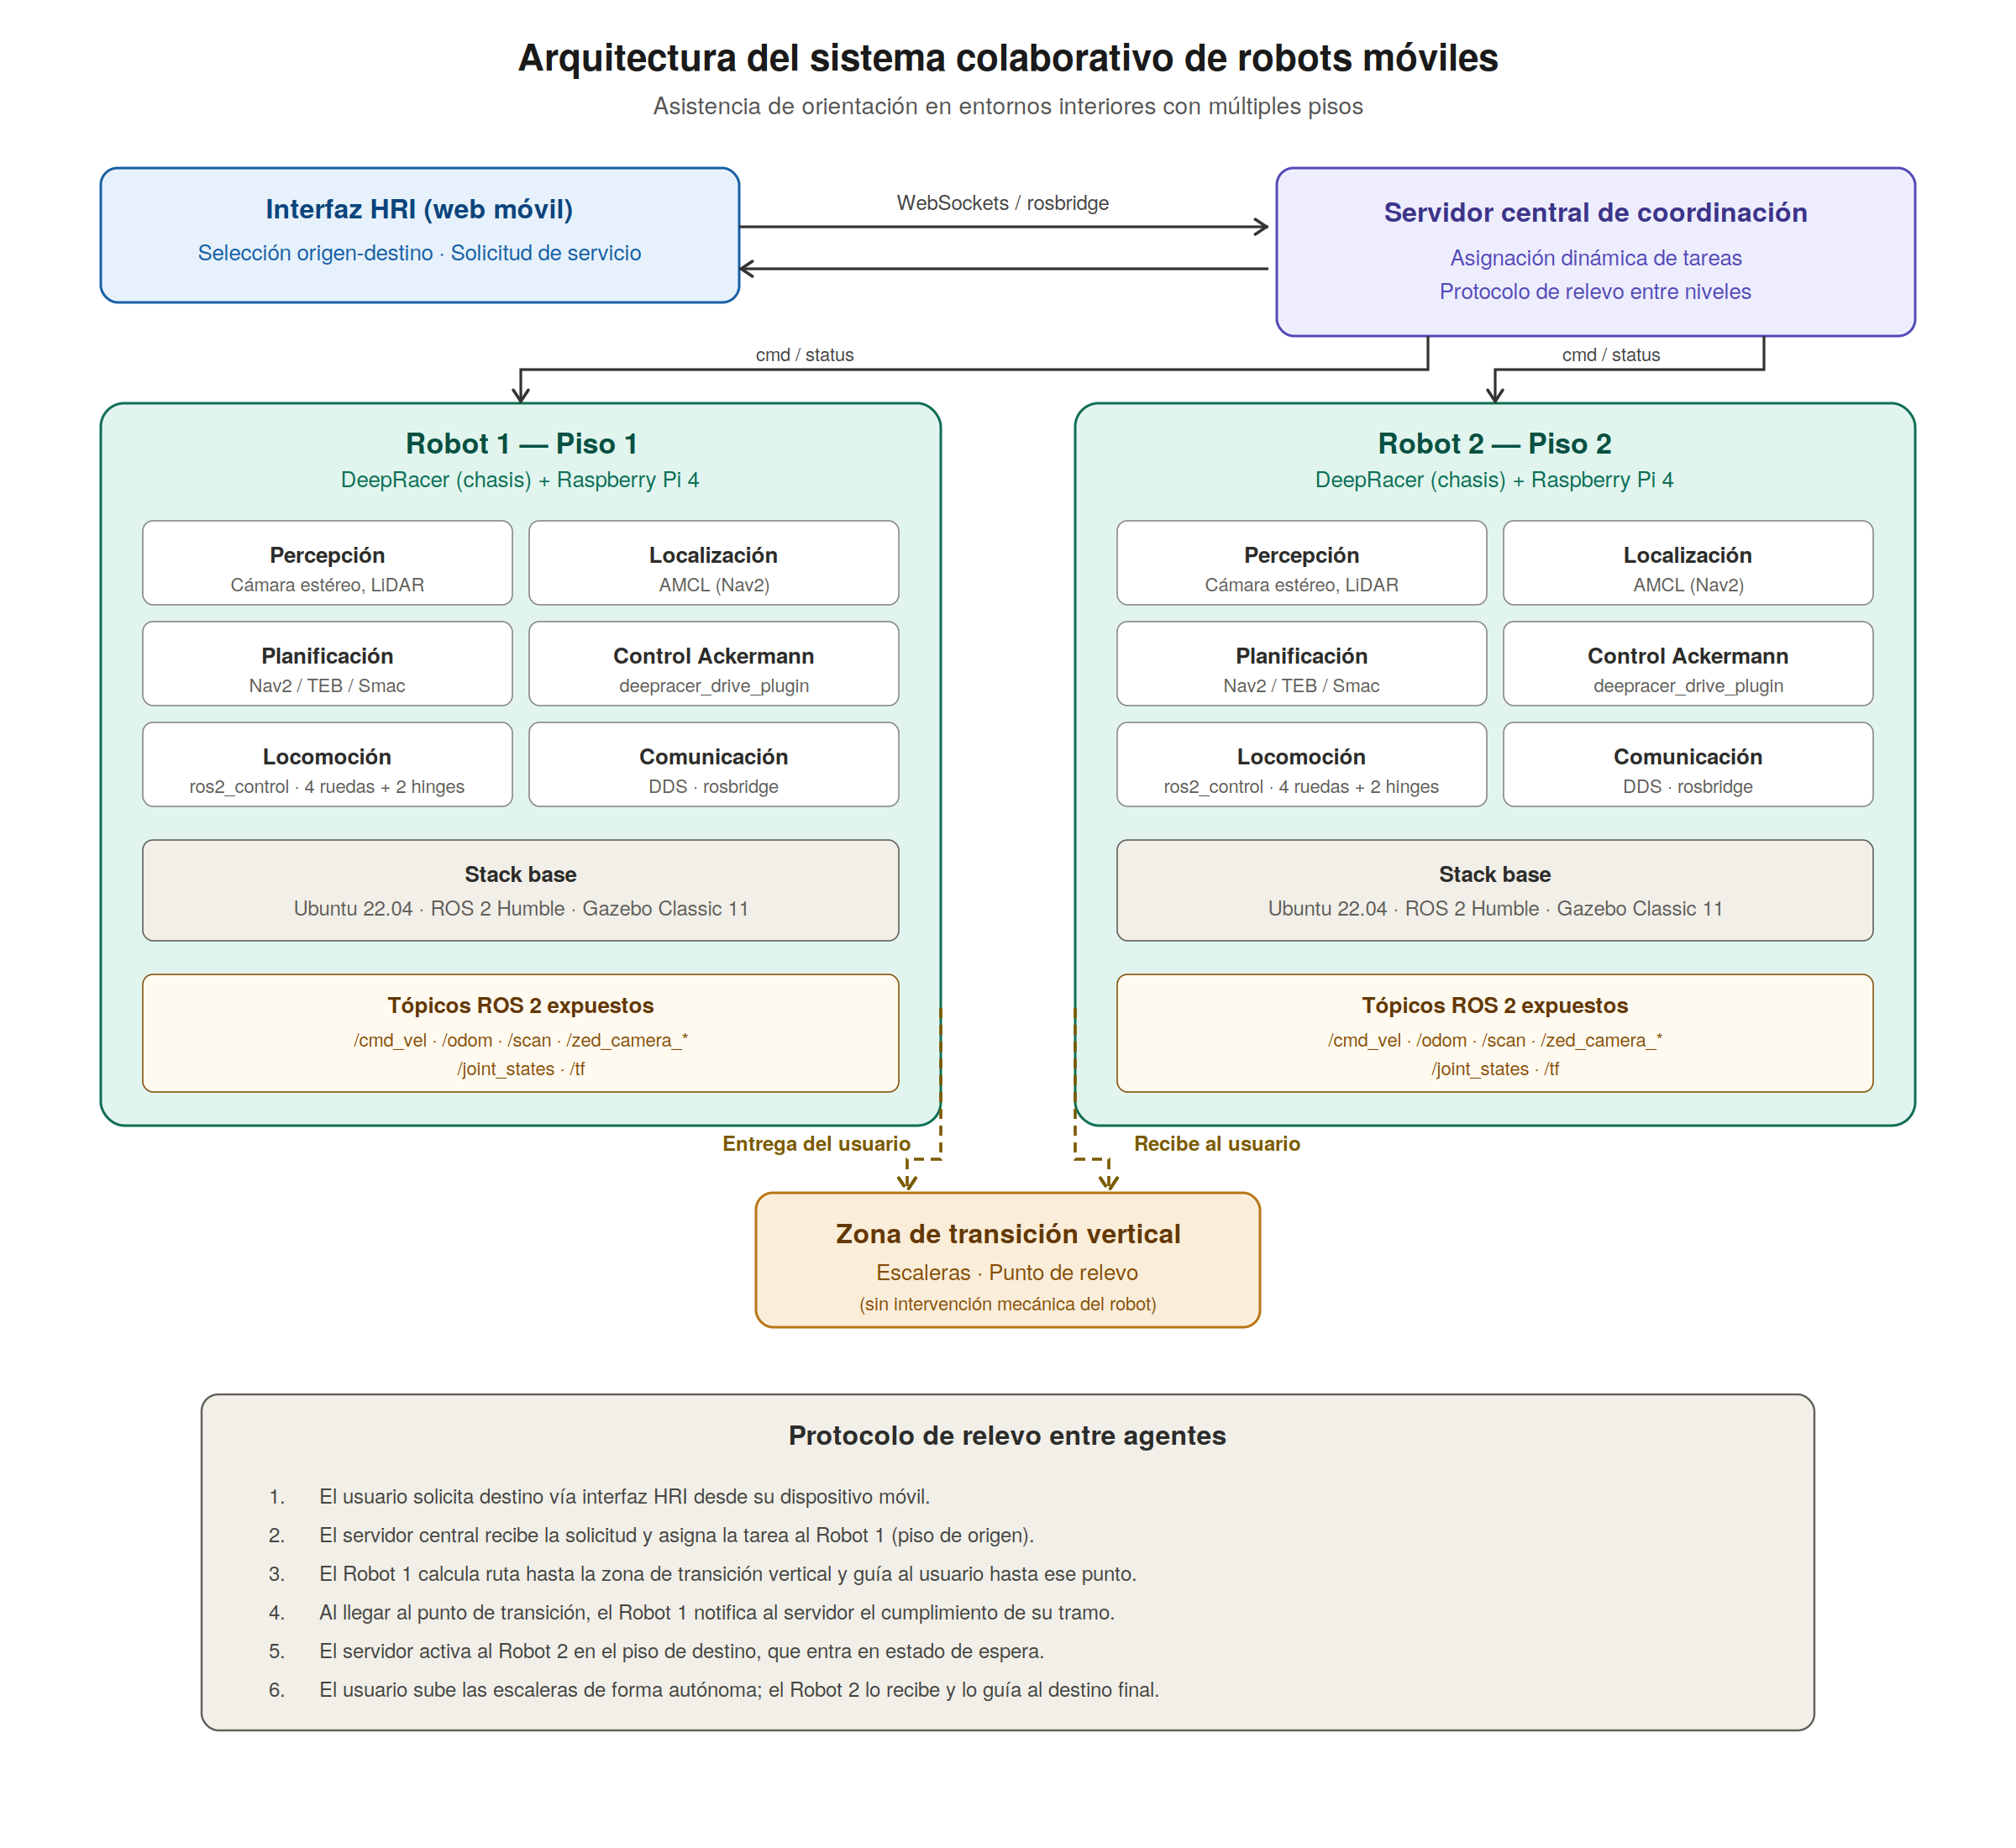
\includegraphics[width=\textwidth]{imagenes/arquitectura_sistema.png}
  \caption{Arquitectura funcional del sistema colaborativo, tal como quedó
    modelada en el OE1. Ningún robot atraviesa la zona de transición: lo que la
    cruza es el usuario, y lo que se traspasa entre agentes es la
    responsabilidad de guiarlo.}
  \label{fig:arquitectura}
\end{figure}

Dos casillas de la figura se concretaron más tarde, y conviene decirlo para que
el lector no las lea como definitivas. La de planificación nombra los candidatos
que se consideraron en el diseño; cuál quedó y por qué está en el §3.2.3. Y los
niveles aparecen como pisos 1 y 2 porque así se planteó el escenario. Al cambiar
de sitio de pruebas pasaron a ser los pisos 3 y 4 (§3.2.5), y la arquitectura no
cambió. Que no cambiara es justamente lo que se esperaba de ella.

\subsection{El contrato de interfaces}

Antes de escribir código se fijó un contrato: qué habla con qué y en qué formato.
El sistema tiene tres piezas. Un \textbf{coordinador} central decide y manda. Dos
\textbf{agentes}, uno por nivel, ejecutan. Y una \textbf{interfaz web} por la que
el usuario pide el servicio.

La comunicación sigue tres reglas que no se rompen:

\begin{enumerate}[leftmargin=*]
  \item El coordinador manda a un agente \textbf{solo} mediante la acción de
    navegación de ROS~2. No publica velocidades directamente.
  \item La interfaz habla \textbf{solo} con el coordinador. Nunca con los
    agentes.
  \item El texto que ve el usuario lo redacta el coordinador. La interfaz lo
    muestra literal.
\end{enumerate}

La tercera evita que la lógica de presentación se duplique en el navegador. Si el
cliente interpretara el estado numérico para decidir qué mostrar, habría dos
copias de la misma lógica y acabarían divergiendo.

\subsection{El planificador, escrito sin ROS a propósito}

El relevo es el aporte declarado del proyecto. Por eso se escribió como función
pura: entran el catálogo de puntos y un par origen-destino, salen los tramos que
hay que ejecutar. No importa el middleware ni mantiene estado.

La razón es de verificabilidad. Si el relevo viviera dentro del nodo, mezclado
con clientes de acción, la única forma de comprobarlo sería levantar dos
simuladores y mirar si el carro llega. Eso es lento y frágil. Como función pura
se agota en milisegundos: \textbf{la prueba recorre 930 combinaciones de
origen-destino y verifica cada plan, sin simulador}.

Esa prueba encontró defectos que una corrida no habría delatado. El más claro:
cuando el origen o el destino \emph{es} el punto de transferencia de su nivel, el
plan mandaba al mismo robot dos veces a la misma pose. Un desplazamiento de cero
metros no falla en Nav2 —devuelve éxito al instante— así que la simulación no lo
habría mostrado.

\subsection{La asignación de tareas}

Cada nivel tiene un robot asignado, y esa correspondencia es un dato de
configuración, no una constante del código. El coordinador elige el agente al
aceptar la solicitud, según el nivel del origen y del destino.

En la taxonomía de \textcite{gerkey2004taxonomy} es una asignación
centralizada e instantánea. Con dos agentes y el nivel decidiendo cuál responde,
un esquema de subasta añadiría complejidad sin dar flexibilidad.

El planificador exige \textbf{exactamente un punto de transferencia por nivel} y
falla con un mensaje explícito si encuentra dos. Hoy cada planta tiene una
escalera y eso se cumple. La verificación está puesta para que el día que haya
dos la decisión se tome a la vista, y no en silencio.

% ---------------------------------------------------------------------
\section{Plataforma robótica (OE2)}

\subsection{Por qué DeepRacer y no DonkeyCar}

El OE2 habla de «dos vehículos tipo DonkeyCar». Los vehículos empleados son dos
AWS DeepRacer, y el cambio conviene explicarlo porque el lector lo va a notar.

DonkeyCar y DeepRacer son la misma clase de plataforma: un chasis de
radiocontrol a escala 1:18 con dirección Ackermann, un computador a bordo y
software abierto. Lo que el objetivo fija —cinemática tipo automóvil, bajo costo,
código modificable— se cumple igual con una que con otra. La diferencia es que la
universidad ya tenía los dos DeepRacer, de modo que usarlos evitó construir
hardware y dejó ese tiempo para el problema que el proyecto declara como suyo,
que es la coordinación.

El cambio no sale gratis y hay que decirlo. El DeepRacer trae su propia pila de
software, pensada para conducción autónoma por visión y para competencia, y buena
parte del trabajo del §3.2.3 consistió en convivir con ella. Un DonkeyCar partiría
de menos capas, pero habría que montarlo.

\subsection{Nav2 sobre un vehículo que no gira sobre su eje}

La plataforma sigue cinemática tipo automóvil. No es holonómica: no puede girar
en el sitio. La configuración por omisión del marco de navegación de ROS~2 asume
tracción diferencial, de modo que propone trayectorias que el vehículo no puede
ejecutar.

Se sustituyeron dos de sus tres capas. La planificación global pasó a un
planificador híbrido A* con modelo Reeds-Shepp, que admite marcha atrás y genera
las maniobras de inversión que el vehículo necesita. El control de seguimiento
pasó a un controlador de persecución pura regulada, con marcha atrás habilitada.
Del árbol de comportamiento se quitó la recuperación que gira sobre el propio
eje, porque el vehículo no puede hacerla.

\subsection{El orden de puesta en marcha}

Cada pieza de la cadena de navegación solo se puede diagnosticar si la anterior
funciona. La guía oficial de puesta en marcha de Nav2 \autocite{nav2setup} lo
plantea como una escalera de siete peldaños. De abajo arriba: transformaciones
entre marcos, odometría, barrido del láser, mapa, localización, mapas de costos
y, al final, planificador y controlador.

El proyecto la siguió en ese orden, y fue lo que permitió aislar el fallo del
apartado siguiente. Sin la escalera, una odometría que no mide se confunde con un
planificador que no planifica, porque los dos se manifiestan igual: el vehículo no
llega. Con ella, el problema queda acotado a un peldaño.

El orden importa además en la ejecución. Los mapas de costos leen el mapa al
configurarse. Si el servidor de mapas no está activo en ese instante, la capa
estática queda vacía. Y entonces el planificador rechaza cualquier meta diciendo
que el punto de partida está ocupado. El mensaje señala el origen, y la causa está tres
peldaños más abajo.

\subsection{La odometría, que fue el cuello de botella}

El vehículo no tiene encoders de rueda. Su única fuente de odometría es la
correspondencia entre barridos sucesivos del láser. Durante meses esa pieza no
funcionó, y el proyecto tardó en entender por qué.

La causa no era de calibración sino de información. En un pasillo recto y de
sección uniforme, cada barrido es prácticamente idéntico al anterior a lo largo
del eje del corredor. El estimador devuelve un desplazamiento cercano a cero y
\emph{acierta}: desde el sensor no ha cambiado nada. Se midió sobre el edificio y
el resultado fue contundente: en los pasillos disponibles la odometría registraba
entre el 5~\% y el 73~\% del avance real.

La figura~\ref{fig:hall} muestra lo que eso produce. Las tres trayectorias son
del mismo vehículo en el mismo hall. La localización se desplaza hasta más de dos
metros respecto de donde el vehículo estaba de verdad, medido con flexómetro, y
en una de las corridas salta fuera del recinto. La línea a trazos marca otro
hallazgo de esa misma sesión: la pared norte estaba modelada 0,84~m más al norte
de lo que está.

\begin{figure}[H]
  \centering
  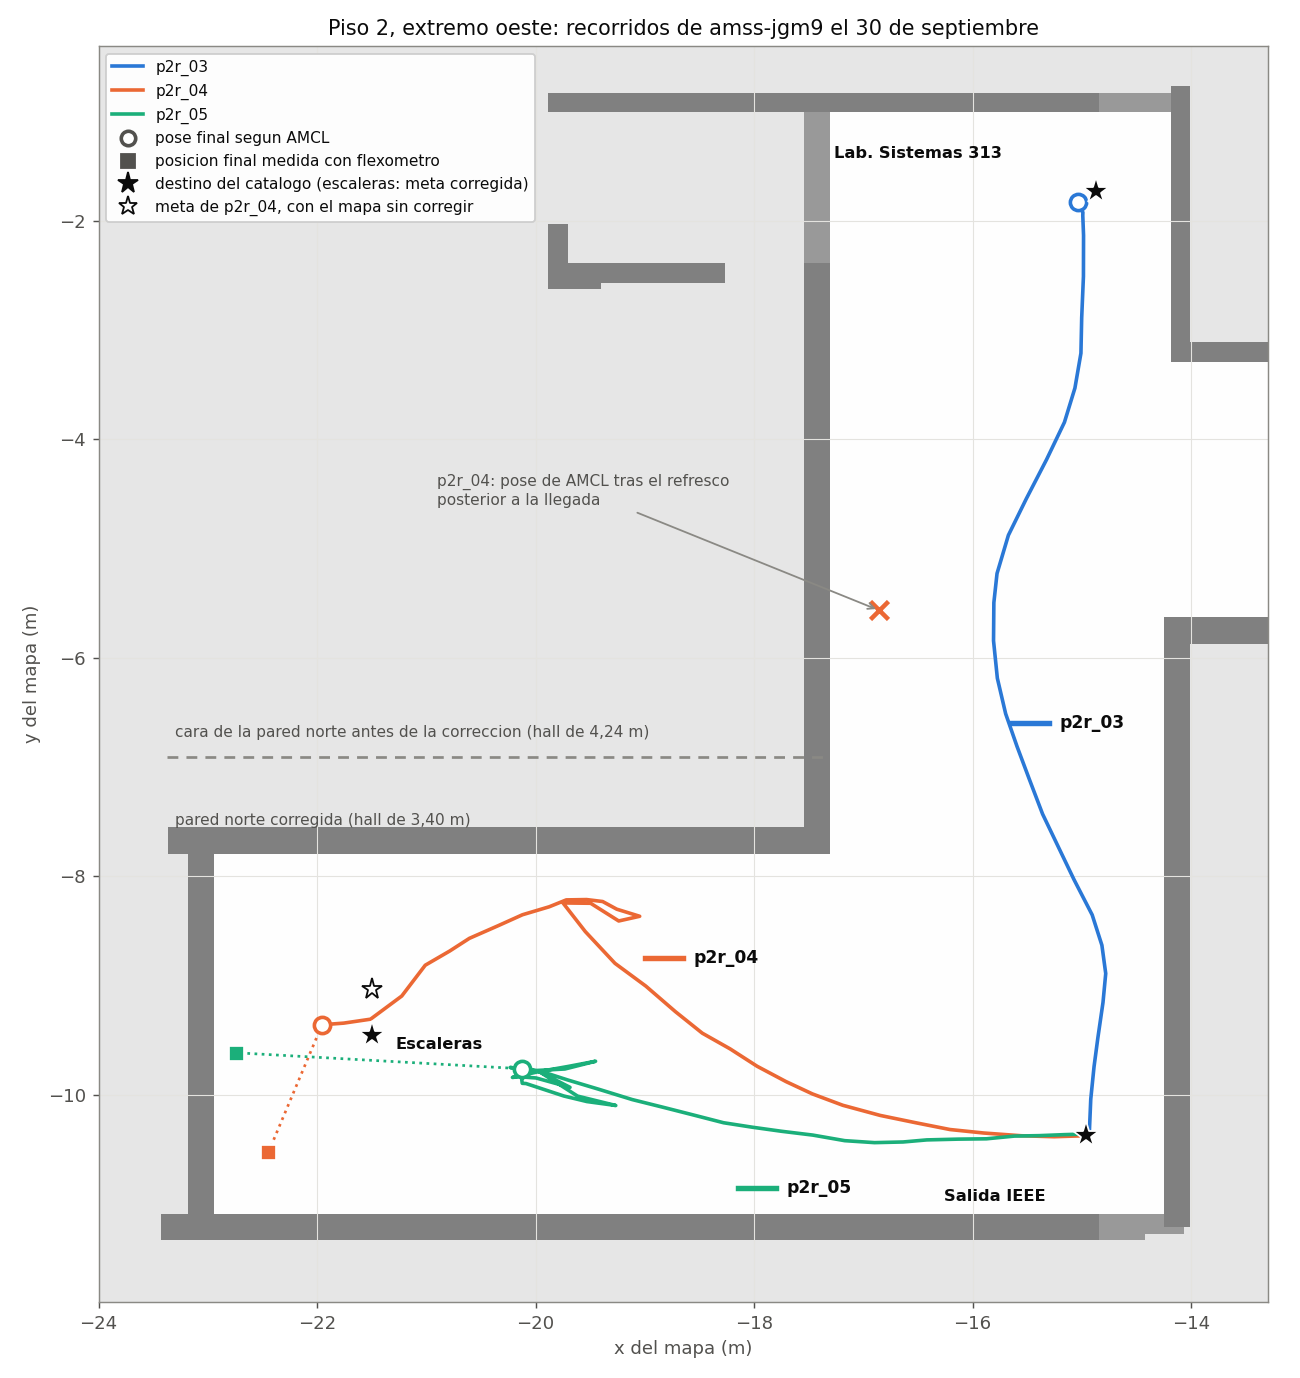
\includegraphics[width=0.78\textwidth]{imagenes/recorridos_hall_piso2.png}
  \caption{Tres recorridos en el hall del piso 2. El círculo es la pose que
    reporta la localización al terminar; el cuadrado, la posición real medida con
    flexómetro. La separación entre los dos es el error, y su causa está en la
    odometría, no en el algoritmo de localización.}
  \label{fig:hall}
\end{figure}

La solución no fue afinar el algoritmo, porque no había nada que afinar. Fue
cambiar de entorno. El criterio para elegirlo salió de la misma medida: hace
falta estructura no uniforme dentro del alcance del sensor durante todo el
recorrido.

Se levantaron con flexómetro dos plantas que la tienen. Entre las tres hornacinas
de salón, los lockers, la papelera, el ascensor y la escalera suman ocho cambios
de perfil en 25~m, uno cada tres metros. Con la misma odometría y sin tocar un
parámetro, el error cayó a menos del 5~\%.

\subsection{Los mapas, derivados de medidas y no de SLAM}

El proyecto intentó durante semanas construir el mapa con SLAM y no lo consiguió
en ningún pasillo, por la misma razón del apartado anterior. La vía que
funcionó fue otra: \textbf{levantar la planta con flexómetro y derivar de ese
levantamiento tanto el mundo simulado como el mapa de navegación}.

Eso tiene una consecuencia que conviene subrayar. Simulación y edificio coinciden
porque salen de la misma fuente, no porque se parezcan. El proyecto había dado
esa correspondencia por supuesta, y al verificarla por primera vez resultó falsa:
el modelo anterior daba un hall 0,84~m más ancho de lo que es, un 20~\% de error.

La herramienta que genera las plantas incluye una comprobación que no se salta.
Un pasillo mide lo mismo por sus dos lados, así que suma las dos paredes y avisa
si no cierran dentro del 2~\%. Esa comprobación encontró cinco errores antes de
generar nada. Las dos plantas cierran al 0,32~\% y al 0,62~\%.

La figura~\ref{fig:mapa4} es el resultado para una de ellas. Lo que se ve no es
un plano dibujado sino el mapa de ocupación con el que navega el vehículo,
generado a partir de las medidas. Los entrantes de los salones, los lockers, el
ascensor y la escalera son los ocho cambios de perfil que hacen observable el
avance.

\begin{figure}[H]
  \centering
  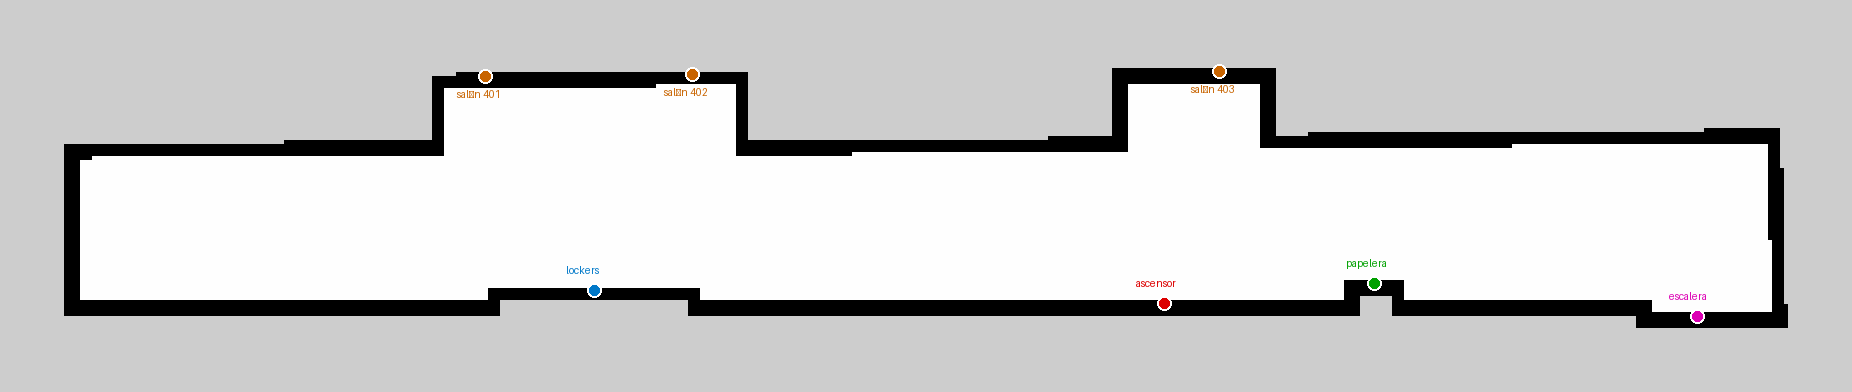
\includegraphics[width=\textwidth]{imagenes/mapa_piso4.png}
  \caption{Mapa de navegación del piso 4, derivado del levantamiento con
    flexómetro. El pasillo corre 25~m del extremo norte al sur; los salones
    quedan al este, y el ascensor y la escalera al oeste.}
  \label{fig:mapa4}
\end{figure}

\subsection{La banda muerta de tracción, y lo que obliga a configurar}

Al integrar la cadena de tracción apareció una característica de la plataforma
que condiciona toda la aproximación al destino. \textbf{El vehículo no se mueve
con velocidad comandada por debajo de 0,40~m/s.} El puente que traduce la orden
de velocidad a la señal del variador la convierte en tracción nula, y lo hace sin
emitir ningún aviso: desde fuera parece que la orden se ejecutó.

Eso forzó una decisión de configuración que conviene dejar escrita, porque tiene
consecuencias. La velocidad mínima de aproximación del controlador se subió a ese
mismo valor, 0,40~m/s. Sin ese ajuste el vehículo se detenía al entrar en la fase
final del recorrido y se quedaba ahí, intentando moverse a una velocidad que su
propia cadena anulaba.

El efecto es que \textbf{el vehículo se aproxima a la meta a 0,40~m/s y no puede
ir más despacio}. No tiene régimen de aproximación fina. Es un límite de la
plataforma, no del software, y no se corrige afinando el controlador: las dos
salidas son bajar el umbral de arranque del vehículo —por mecánica o por
calibración de los servos— o fijar la tolerancia de llegada en un valor
compatible con la plataforma, con justificación previa. Las dos son decisiones,
no ajustes, y por eso quedan planteadas en el capítulo de trabajos futuros.

% ---------------------------------------------------------------------
\section{Interfaz humano-robot (OE3)}

\subsection{Una página web, no una aplicación}

El OE3 pide «una interfaz móvil». Lo que se construyó es una página web que se
abre en el navegador del teléfono. Cumple el objetivo: es móvil porque se usa
desde el teléfono del usuario. Y lo cumple mejor que una aplicación nativa. Un
visitante ocasional —que es el usuario que el proyecto declara— no va a instalar
nada para preguntar por un salón.

El requisito pedía que el usuario no instalara nada. La interfaz es una página
web que se abre desde el navegador del teléfono. No usa recursos externos,
porque debe funcionar sin salida a internet: en la red del edificio puede no
haberla.

La comunicación con el middleware pasa por un puente que expone las acciones de
ROS~2 como JSON sobre WebSocket. La librería de cliente más difundida del
ecosistema no servía: su cliente de acciones corresponde a la generación anterior
del middleware y es incompatible. La interfaz usa por eso un cliente propio,
escrito directamente sobre el protocolo del puente.

\subsection{Lo que el usuario ve}

El usuario elige origen y destino de un catálogo con búsqueda por nombre, y pulsa
un botón. A partir de ahí la página muestra el estado de la misión con el texto
que redacta el coordinador.

Dos funciones se añadieron después de ver el sistema en uso:

\textbf{Confirmación de cambio de piso.} La secuencia de una misión entre niveles
termina la etapa de transferencia cuando el robot del piso de destino llega a su
escalera. Pero el robot no puede saber si \emph{la persona} ya subió. Sin una
pausa explícita, la misión podía declararse completada con el usuario todavía en
el piso equivocado, y la instrumentación lo habría registrado como éxito.

\textbf{Cancelación.} El botón existía pero no hacía nada, y nadie lo había
notado: el servidor de acción no registraba la función de cancelación, de modo
que el middleware rechazaba toda solicitud por omisión y en silencio. Al
corregirlo se añadió además el comportamiento que faltaba: al cancelar, el robot
en curso regresa a su escalera antes de que la misión cierre.

% ---------------------------------------------------------------------
\section{Protocolo experimental (OE4)}

El protocolo se escribió \textbf{antes} de instrumentar el sistema, y esa
secuencia es deliberada. Fija las cuatro métricas con definición operativa, el
criterio de éxito, el tamaño de muestra y una lista cerrada de causas de
descarte con su techo.

Dos decisiones del protocolo merecen mención porque condicionan cómo se leen los
resultados.

La primera: \textbf{el éxito se mide contra la odometría del vehículo, nunca
contra el resultado que devuelve Nav2}. Una navegación puede terminar en
\emph{éxito} y haber dejado al robot lejos del destino. Aceptar ese resultado
sería dejar que el sistema se evalúe a sí mismo.

La segunda: \textbf{las misiones se sortean}. Con pares elegidos a mano se corre
el riesgo de probar justo los recorridos que funcionan.

Durante la escritura del analizador apareció un defecto que ninguna corrida
habría revelado, y que se trata en el §\ref{sec:limitaciones}: uno de los
criterios estaba formulado de manera que no podía dar resultado negativo.

% =====================================================================
%  RESULTADOS
%  Cifras de RESULTADOS_OE4_SIMULACION.md y de la evidencia de hardware
%  S24_peldano2 / S24_nav2_navegacion / S25_pisos34_campo.
%
%  Las tres cosas que hay que escribir con cuidado van en §4.4:
%   - R14: la continuidad es un invariante, no un resultado experimental
%   - El intervalo de Wilson: «supera el 70 %», no «es del 86,7 %»
%   - R15: la campaña corrió con un mapa que leía libre lo desconocido
% =====================================================================
\chapter{Resultados}

\begin{notaavance}[la toma de datos cierra el 16 de octubre de 2026]
Las cifras de este capítulo son las disponibles al \textbf{5 de octubre de
2026}. Las dos mitades están en situaciones distintas y conviene no leerlas
igual:

\begin{itemize}[leftmargin=*,nosep]
  \item El §4.1, \textbf{simulación}, está \textbf{cerrado}. La campaña de
    treinta misiones corrió el 5 de septiembre, el analizador la dictaminó
    válida y sus números no van a cambiar.
  \item El §4.2, \textbf{hardware}, \textbf{va por mitades}. La odometría
    (compuerta G-2) cerró el 5 de octubre y se reporta. La precisión de llegada
    (G-3) no se alcanzó en el corte C-1 y sigue abierta, así que ese apartado
    queda sin redactar hasta el corte del \textbf{viernes 16 de octubre},
    después del cual el acta de directores no admite más datos.
\end{itemize}

El §4.3 trata de las limitaciones de la campaña de simulación, así que cierra
con ella.
\end{notaavance}

Los resultados llegan de dos campañas distintas. La primera, en simulación, con
treinta misiones sorteadas. La segunda, sobre los vehículos reales en los
pasillos del edificio. Se reportan por separado porque miden cosas distintas: la
de simulación mide el sistema completo con relevo, la de hardware mide hasta
dónde llega la plataforma física.

% ---------------------------------------------------------------------
\section{Evaluación en simulación}

La campaña corrió treinta misiones sorteadas, quince de control dentro de un
mismo nivel y quince entre niveles. El analizador dictaminó \textbf{campaña
válida}, con \textbf{cero descartes} contra un techo admitido del 20~\%.

\subsection{Tasa de éxito (RF-23)}

Una misión es exitosa si cumple dos cosas. Que la pose final quede a 0,25~m o
menos del destino, medida contra la odometría y no contra el resultado de Nav2.
Y que la misión llegue a completarse sin pasar por fallo.

\begin{table}[H]
  \centering\small
  \caption{Tasa de éxito de la campaña, con intervalo de confianza de Wilson.}
  \label{tab:exito}
  \begin{tabular}{@{}lcccc@{}}
    \toprule
    & \textbf{n} & \textbf{éxitos} & \textbf{tasa} & \textbf{IC 95 \% (Wilson)} \\ \midrule
    Campaña completa & 30 & 26 & \textbf{86,7 \%} & \textbf{70,3 -- 94,7 \%} \\
    Condición A — control & 15 & 12 & 80,0 \% & 54,8 -- 93,0 \% \\
    Condición B — inter-nivel & 15 & 14 & 93,3 \% & 70,2 -- 98,8 \% \\ \bottomrule
  \end{tabular}
\end{table}

\textbf{La afirmación defendible es que la tasa de éxito supera el 70~\%}, no que
sea del 86,7~\%. Con treinta misiones el intervalo mide 24 puntos porcentuales de
ancho, y ese límite es de diseño: no se arregla trabajando más, se arreglaría con
más muestra. El 86,7~\% es el estimador puntual y se reporta siempre junto a su
intervalo.

Los dos intervalos de las condiciones se solapan, así que \textbf{la comparación
entre ellas no sostiene ninguna conclusión}. Conviene decirlo porque el estimador
puntual apunta en contra de la intuición: la condición con relevo salió mejor que
la de control.

\subsection{Los cuatro fallos son un solo modo}

Las cuatro misiones fallidas quedaron a 0,295, 0,284, 0,311 y 0,347~m del
destino, contra una tolerancia de 0,25~m. Las cuatro se quedaron \emph{cortas},
ninguna se pasó ni terminó en otro sitio.

Eso no es un fallo de coordinación: es el límite de precisión de la aproximación
final. El error de llegada del conjunto tiene mediana \textbf{0,106~m} y recorrido
de 0,019 a 0,347~m.

\subsection{Tiempo de respuesta (RF-21) y de asignación (RF-22)}

El tiempo de respuesta se reporta por escalones y no con media y desviación, por
una razón de instrumento:

\begin{table}[H]
  \centering\small
  \caption{Tiempo de respuesta, en escalones del reloj de simulación.}
  \label{tab:respuesta}
  \begin{tabular}{@{}lcccc@{}}
    \toprule
    \textbf{t respuesta} & 0,1 s & 0,2 s & 0,3 s & 0,4 s \\ \midrule
    misiones & 10 & 15 & 4 & 1 \\ \bottomrule
  \end{tabular}
\end{table}

Los cuatro valores son múltiplos exactos de 100~ms, que es el tic del reloj de
simulación. \textbf{La resolución del instrumento vale entre el 25~\% y el 100~\%
de la magnitud medida.} Una mediana de 0,2~s significa «uno o dos tics», no
«doscientos milisegundos». Dar media y desviación sugeriría una precisión que el
reloj no entrega.

Lo que sí se sostiene es la cota, que además es lo que le importa a un usuario:
\textbf{el robot arranca en menos de medio segundo}.

El tiempo de asignación quedó por debajo de 100~ms en las treinta. Como esa cifra
cae tres órdenes de magnitud por debajo de un tic del reloj, se caracterizó
aparte en banco: mediana entre 154 y 175~\textmu s, máximo 306~\textmu s.

% ---------------------------------------------------------------------
\begin{figure}[H]
  \centering
  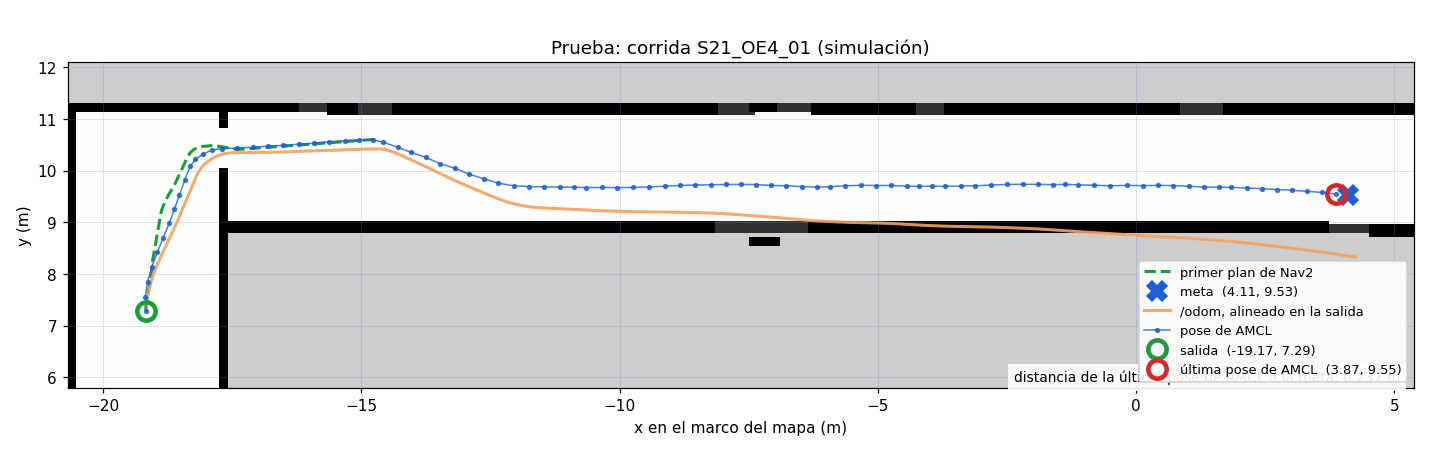
\includegraphics[width=\textwidth]{imagenes/corrida_simulacion.png}
  \caption{Una misión de la campaña en simulación. Se superponen el primer plan
    que calcula el navegador, la pose estimada a lo largo del recorrido y la
    odometría cruda. La separación creciente entre las dos últimas es la deriva
    que la localización corrige contra el mapa.}
  \label{fig:simulacion}
\end{figure}

\section{Evaluación sobre hardware}

\begin{notaavance}[G-2 cerrada el 5 de octubre; G-3 sigue abierta]
De las dos compuertas que esta sección tiene que responder, una cerró y la otra
no, así que se reportan de forma distinta:

\begin{itemize}[leftmargin=*,nosep]
  \item \textbf{G-2, la odometría}, quedó \textbf{alcanzada} en el acta de
    directores del 5 de octubre de 2026, con las medidas del 2 de octubre en el
    piso 4. Sus cifras son definitivas y se reportan en el §4.2.1.
  \item \textbf{G-3, la precisión de llegada}, \textbf{no se alcanzó} en el
    corte C-1 y sigue abierta. El §4.2.2 queda sin redactar: la toma de datos
    continúa hasta el corte del \textbf{16 de octubre}, y escribir ahora unas
    cifras que van a cambiar obligaría a corregirlas después.
\end{itemize}
\end{notaavance}

\subsection{La odometría del vehículo (G-2)}

El vehículo no tiene encoders, así que su odometría sale de comparar barridos
sucesivos del láser. Durante meses esa pieza no produjo una medida utilizable.
La tabla~\ref{tab:odometria} reúne lo que se midió en cada entorno:

\begin{table}[H]
  \centering\small
  \caption{Fracción del avance real que registra la odometría, por entorno.}
  \label{tab:odometria}
  \begin{tabular}{@{}lccl@{}}
    \toprule
    \textbf{Entorno} & \textbf{Recorrido} & \textbf{Registrado} & \textbf{Criterio $\pm$10 \%} \\ \midrule
    Pasillo simulado, 46,9 m & largo & 37,9 \% & falla \\
    Pasillos del edificio (piso 1 y 2) & largo & 5,7 \% y 1,3 \% & falla \\
    Hall del piso 2 & 6 m & 73 \% & falla \\
    Cuarto cerrado, empujado a mano & 3 m & 96,3 -- 101,9 \% & \textbf{cumple} \\
    \textbf{Pasillo del piso 4} & \textbf{6,68 m} & \textbf{95,4 \%} & \textbf{cumple} \\
    \textbf{Pasillo del piso 4} & \textbf{14,57 m} & \textbf{103,3 \%} & \textbf{cumple} \\ \bottomrule
  \end{tabular}
\end{table}

La lectura importa más que las cifras. \textbf{El estimador no mejoró: cambió el
entorno.} En un pasillo recto y uniforme la información de avance no está en el
dato del sensor, y ningún ajuste la recupera. En un pasillo con hornacinas,
lockers y quiebres —ocho cambios de perfil en 25~m— la misma odometría, sin tocar
un parámetro, queda dentro del $\pm$5~\%.

Sobre esas dos últimas filas, las del piso 4, los directores declararon
\textbf{G-2 alcanzada}. Es la compuerta que el proyecto llevaba desde septiembre
señalando como su única ruta crítica.

\subsection{La navegación y la precisión de llegada (G-3), pendientes}

\begin{notaavance}[apartado sin redactar: la toma de datos cierra el 16 de
octubre de 2026]
Aquí irán dos cosas, y ninguna se adelanta:

\begin{enumerate}[leftmargin=*,nosep]
  \item \textbf{La navegación}: evidencia, a partir del registro de cada
    corrida, de que el planificador traza y el controlador sigue sobre el
    vehículo real.
  \item \textbf{La precisión de llegada} (G-3): distancia medida con flexómetro
    entre la parada del vehículo y el destino del catálogo, contra la tolerancia
    de 0,5~m que fijó el director.
\end{enumerate}

Hay sesiones de campo realizadas y sus medidas están registradas en el
repositorio, pero \textbf{no se reportan todavía como resultado}: G-3 no se
alcanzó en el corte C-1 y la demostración continúa. Lo que haya el 16 de octubre
es lo que se defiende.

Lo que sí está medido, y no depende de cuántas corridas más se hagan, es el
mecanismo que condiciona esa llegada: la banda muerta de tracción del vehículo,
documentada en el §3.2.6.
\end{notaavance}

\section{Limitaciones de la medición}
\label{sec:limitaciones}

Tres límites afectan a cómo deben leerse los resultados anteriores. Se declaran
aquí porque callarlos sería presentar como medida lo que no lo es.

\subsection{La continuidad entre niveles es un invariante, no un resultado}

La continuidad del servicio es la variable de respuesta principal del objetivo~4,
y su criterio binario se cumplió en las treinta misiones. \textbf{Ese resultado no
es evidencia de nada}, y la razón es estructural.

El criterio exige que dentro de la ventana de la misión el coordinador nunca esté
en estado inactivo y nunca tenga el agente sin asignar. Los dos únicos puntos del
código que producen esos valores ocurren \emph{antes} de que la ventana se abra.
No existe ejecución posible que lo incumpla: son cero incumplimientos de cero
posibles.

Un criterio que no puede dar resultado negativo no aporta evidencia, por muchas
veces que se verifique. La corrección no fue inventar una ruta de fallo. Eso habría sido instrumentar el
experimento para que pareciera más informativo. Lo que se hizo fue
\textbf{declarar la continuidad como invariante estructural del diseño} y apoyar
la afirmación en una magnitud que sí varía: el hueco temporal del relevo. En las
quince misiones entre niveles tuvo mediana de 0,1~s y máximo de 0,2~s.

\subsection{El intervalo de confianza es ancho por diseño}

Ya se dijo en la tabla~\ref{tab:exito} y se repite porque es el límite más fácil
de olvidar al redactar: con treinta misiones, \textbf{lo defendible es una cota
inferior}, no un valor puntual. Aumentar la confianza exige más muestra, no más
trabajo.

\subsection{El mapa de la campaña leía como libre lo desconocido}

El mapa con que corrió la campaña declaraba un umbral que hacía que
\textbf{10\,908 celdas desconocidas —el 14,5~\% del mapa— se cargaran como
espacio libre}. Con ello, las dos salvaguardas que debían impedir planificar
sobre lo no explorado quedaban desactivadas de hecho.

El alcance de la afirmación, y no más: esto \textbf{no invalida el veredicto}. Los
cuatro fallos fueron de precisión de llegada, no de trazado, y el pasillo por el
que se navegó está mapeado como libre de verdad. Lo que no se sabe es si alguna
trayectoria cruzó una de esas celdas, y es comprobable sobre los registros
conservados. El defecto está corregido desde el 25 de septiembre.

% =====================================================================
%  CONCLUSIONES
%  La plantilla admite dos formas: un párrafo por objetivo específico, o un
%  párrafo denso que evidencie el cumplimiento de los específicos y con ellos
%  el general. Con cuatro OE rastreados uno a uno en REQUISITOS.md, la primera
%  forma es la que menos margen deja a la vaguedad.
% =====================================================================
\chapter*{Conclusiones}
\addcontentsline{toc}{chapter}{CONCLUSIONES}

% PENDIENTE

% =====================================================================
%  TRABAJOS FUTUROS
% =====================================================================
\chapter*{Trabajos futuros}
\addcontentsline{toc}{chapter}{TRABAJOS FUTUROS}

\begin{notaavance}[lista sujeta a lo que arroje la campaña física]
Esta lista se cierra cuando cierre la toma de datos, el 16 de octubre de 2026.
Las cuatro líneas que siguen salen de límites ya medidos y no van a
desaparecer; lo que puede ocurrir es que las sesiones que faltan añadan alguna
más.
\end{notaavance}

Las líneas que siguen salen de límites concretos que el trabajo encontró y
documentó, no de una lista genérica de mejoras.

\textbf{Resolver la aproximación fina del vehículo.} Es la limitación que impide
cumplir la tolerancia de llegada, y está localizada. El vehículo no se mueve por
debajo de 0,40~m/s: la cadena de tracción traduce esa velocidad a cero. Hay
dos vías. Una es de hardware —calibrar los servos o cambiar la relación de
transmisión— y daría al vehículo un régimen lento del que hoy carece. La otra es
de criterio: fijar la tolerancia de llegada a un valor compatible con la
plataforma, con justificación previa y no a la vista de los resultados.

\textbf{Añadir una fuente de odometría independiente del láser.} La odometría
actual deduce el movimiento comparando barridos, y eso falla por construcción en
pasillos uniformes. El proyecto lo resolvió eligiendo un entorno con estructura,
pero esa solución limita dónde puede operar el sistema. Una unidad inercial, o
odometría visual con las cámaras que los vehículos ya llevan, daría información
de avance que no depende de la geometría del sitio.

\textbf{El ascensor como segunda vía de transición.} Hoy el cambio de piso se
hace siempre por la escalera, y el ascensor es un destino más. Admitir los dos
exige que el planificador elija entre dos puntos de transferencia por nivel,
presumiblemente el más cercano al punto anterior. El código ya nombra esa
decisión y falla explícitamente cuando encuentra dos, de modo que el punto de
extensión está identificado.

\textbf{Resolver una esquina.} Todos los recorridos medidos fueron sobre tramos
rectos. El guiado real tiene esquinas. El controlador demostró mover la dirección, pero
no se ha probado que el vehículo resuelva un cambio de rumbo grande en un pasillo
estrecho. Un intento de media vuelta en un corredor de 2,3~m no fue
posible.

\textbf{Ampliar la muestra de la campaña.} Con treinta misiones el intervalo de
confianza mide 24 puntos porcentuales. Ese ancho es de diseño y solo se reduce
con más repeticiones. Una campaña mayor permitiría además comparar las dos
condiciones experimentales, cosa que hoy no se sostiene porque sus intervalos se
solapan.

\textbf{Operar con los dos vehículos en el mismo grafo.} Las pruebas de hardware
se hicieron con un vehículo cada vez, porque los dos publican en los mismos
nombres de tópico y una orden alcanza a ambos. Separarlos por espacio de nombres
está diseñado y probado en el computador, pero no ejercitado en campo, y es
condición para la demostración del sistema completo.


% =====================================================================
%  REFERENCIAS
% =====================================================================
\ustaseccion{Referencias bibliográficas}
\printbibliography[heading=none]

\end{document}
